\documentclass{Supervised_Reinforcement_Learningqsport}
\usepackage{graphicx}
\usepackage{float}
\usepackage{cite}
\usepackage{amsmath,amssymb,amsfonts}
\usepackage{algorithmic}
\usepackage{graphicx}
\usepackage{textcomp}
\usepackage{xcolor}
\usepackage[utf8]{inputenc} % Input encoding

\begin{document}

\title{Traffic Signal Control with Deep Reinforcement Learning}

\author{José Alfredo Zapana García
\thanks{José Alfredo Zapana García¸
Faculdade de Engenharia Elétrica e de Computação (FEEC), Universidade Estadual de Campinas (UNICAMP), Campinas-SP. E-mails: j272291@dac.unicamp.br.}}

\maketitle

\markboth{IA368 - APRENDIZADO POR REFORÇO - 2024-1º SEMESTRE} {IA368 - APRENDIZADO POR REFORÇO - 2024-1º SEMESTRE}

\begin{resumo}
Este documento apresenta um exemplo de utilização de um estilo \LaTeX\ que produz uma boa aproximação do estilo \textit{IEEEtran.cls} adotado nas conferências do IEEE.
\end{resumo}

\section{Proposition}

\subsection{Problem Description}

Optimize traffic signal control to reduce vehicle waiting and enhance overall traffic flow efficiency

Traffic dynamics is a non-linear problem that is difficult to model.

Stochastic and non-linear nature of traffic flow. 

There have been efforts to use Reinforcement Learning with a Model-Free approach to train a model to control the traffic lights of intersections.

As noted by [REFS], choosing a correct reward signal is fundamental for the agent to find an optimal policy, rewards such as queue length, average speed, total waiting time, 

\begin{figure}[htbp]
   \centerline{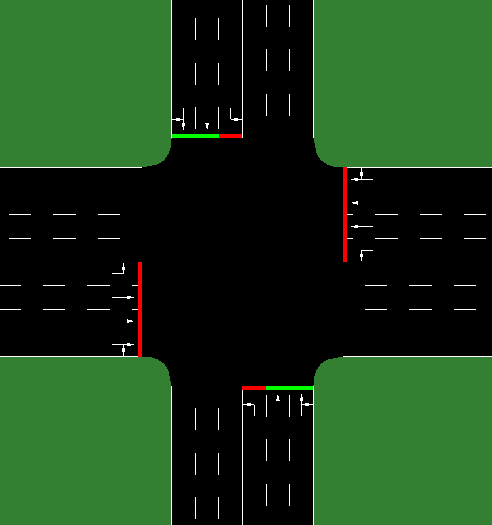
\includegraphics[width=0.6\columnwidth]{snap_envSUMO.png}}
    \caption{Snapshot of the traffic environment.}
    \label{fig:snap}
\end{figure}

\subsection{Methods and Current Implementation}

The two most common approaches will be compared: Q-value methods and Policy Optimization Methods, to see which of these is better with this type of problem.

Currently, there an implementation of Rainbow DQN 

The current implementation is located at GitHub link [To Replace].

\begin{thebibliography}{99}

\bibitem{ref1} Y. Han, M. Wang, and L. Leclercq, “Leveraging reinforcement learning for dynamic traffic control: A survey and challenges for field implementation,” Commun. Transp. Res., vol. 3, no. November, 2023, doi: 10.1016/j.commtr.2023.100104.
\bibitem{ref2} H. Wei, G. Zheng, V. Gayah, and Z. Li, “Recent Advances in Reinforcement Learning for Traffic Signal Control,” ACM SIGKDD Explor. Newsl., vol. 22, no. 2, pp. 12–18, 2021, doi: 10.1145/3447556.3447565.
\bibitem{ref3} C.-C. Chao, J.-W. Hsieh, and B.-S. Wang, “Cooperative Reinforcement Learning on Traffic Signal Control,” vol. XX, no. Xx, pp. 1–10, 2022, [Online]. Available: http://arxiv.org/abs/2205.11291.
\bibitem{ref4} L. Huang and X. Qu, “Improving traffic signal control operations using proximal policy optimization,” IET Intell. Transp. Syst., vol. 17, no. 3, pp. 592–605, 2023, doi: https://doi.org/10.1049/itr2.12286.
\bibitem{ref5} Y. Shi, Z. Wang, T. J. LaClair, C. Wang, Y. Shao, and J. Yuan, “A Novel Deep Reinforcement Learning Approach to Traffic Signal Control with Connected Vehicles †,” Appl. Sci., vol. 13, no. 4, 2023, doi: 10.3390/app13042750.
\bibitem{ref6} O. Chergui and L. Sayad, “Mitigating congestion in multi-agent traffic signal control: an efficient self-attention proximal policy optimization approach,” International Journal of Information Technology (Singapore), vol. 16, no. 4. pp. 2273–2282, 2024, doi: 10.1007/s41870-023-01545-8.
\bibitem{ref7} A. Fontoura, D. B. Haddad, and E. Bezerra, “A Deep Reinforcement Learning Approach to Adaptive Traffic Lights Management,” Proc. - 2019 Brazilian Conf. Intell. Syst. BRACIS 2019, no. Woa, pp. 216–221, 2019, doi: 10.1109/BRACIS.2019.00046.
\bibitem{ref8} H. Luo, Y. Bie, and S. Jin, “Reinforcement Learning for Traffic Signal Control in Hybrid Action Space,” IEEE Trans. Intell. Transp. Syst., vol. PP, pp. 1–17, 2024, doi: 10.1109/TITS.2023.3344585.

\end{thebibliography}

\end{document}
